\section{Middleware Architecture}

\subsection{Server Architecture}

The company architecture contains the following components: Client Application, Middleware server, Middleware Cache, Metadata Server and Content Servers. The brief architecture overview is presented on figure \ref{fig:arch_overview}. 


\begin{figure}[h]
    \centering
	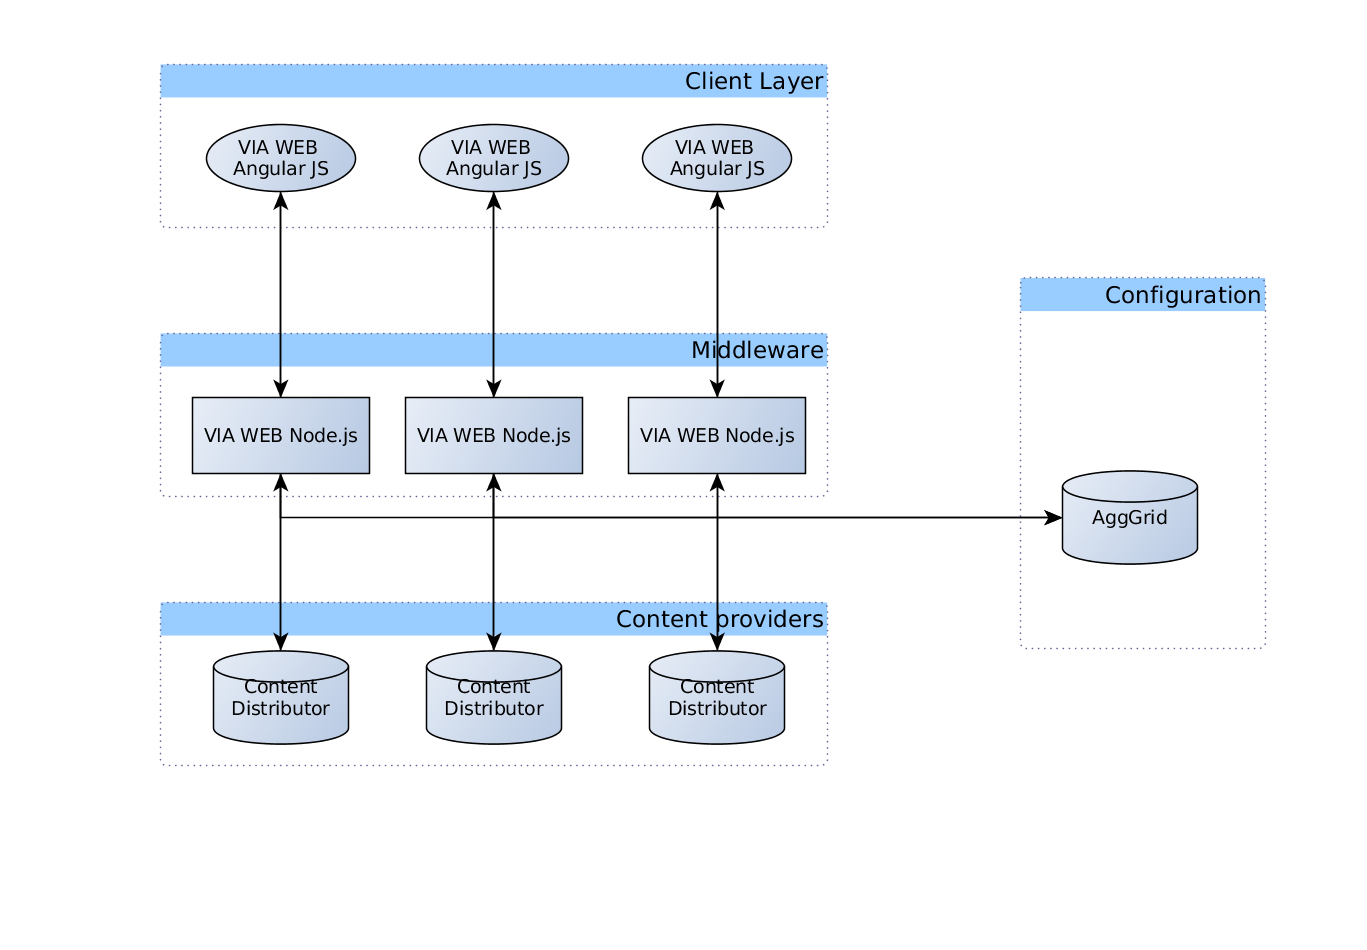
\includegraphics[width=\textwidth]{images/thesis_global_architecture_existing.png}
    \caption{Global architecture overveiw}
    \label{fig:arch_overview}
\end{figure}


The client is a web application developed using Javascript, HTML, CSS framework and Model View Controller pattern. It communicates with middleware server through REST services based on HTTP protocol. The client has several components: Controllers, Managers, Services. 

The contollers validate the user data, invoke corresponding managers and render data to the view objects represented by HTML pages. The managers are implemented using Facade pattern\cite{DesignPatterns}. They hold and manage services, construct View Model Objects from service responses and send them back to controllers. 

The services are communication layer between the client application and the middleware server. They communicate via REST services based on HTTP protocol. This brings flexibility to the architecture and makes components loosely coupled.[describe why it is good?]. 

The middleware server serves as a data aggregator and security point. It translates requests from the client application to the format understandable by the metadata server or content distributors, gathers data from content distributors, builds data model objects(the definition is given in the next section) and sends the as JSON entities to the client application.

Content servers(content distributors) are customer servers. They are the main sources of information that needs to be presented by the client application. They can be represented for example by the movie entities or music distributors.

The metadata server is the company developed server that stores and processes auxiliary and configurational information. The requests can be: 

\begin{itemize}
	\item Data aggregation - required fo analytical purposes
	\item User action logs 
	\item User settings - specific user settings, for example watch history for movie entities.
	\item Client and midldeware configuration
\end{itemize} 

The interaction between components can be described as following: the client application initiates the process by  sending requests to the middleware server. The middleware server redirects requests to the underlying servers(content distributors or metadata server), builds data model objects, and sends them to the client application. The client request can be one of two types, configurational or data demand. If the request is configurational the middleware server redirects it to the metadata server, otherwise it redirects the request to the Content server. The middleware supports local cache and caches every response that is not assosiated with the user session or unique and private user data. The message diagram between architecture components is depicted on figure \ref{fig:arch_uml}.


\begin{figure}[h]
\begin{center}

	\resizebox{1.0\textwidth}{0.8\textwidth} {

	\begin{sequencediagram}
	\newthread[white]{cl}{Client}
	\newinst[1.7]{mw}{Middleware}
	\newinst{lc}{Local Cache}
	\newinst[1.9]{ms}{Metadata Server}
	\newinst[1.3]{cs}{Content Server}

	\begin{call}{cl}{First request}{mw}{Response}

		\begin{call}{mw}{Create new session}{ms}{Session ID}
		\end{call}

		\begin{call}{mw}{Cache Session}{lc}{}
		\end{call}

		\begin{call}{mw}{Get content locator}{ms}{URL}
		\end{call}

		\begin{call}{mw}{Cache Locator}{lc}{}
		\end{call}

	\end{call}

	\begin{call}{cl}{GET Request}{mw}{GET Response}
		
		\begin{call}{mw}{Check Local Cache}{lc}{}
		\end{call}

		\begin{sdblock}{alt}{if data in cache}
			\begin{call}{mw}{Send response to Client}{cl}{}
			\end{call}
			\begin{sdblock}{else}{}
				\begin{call}{mw}{Request Content}{cs}{Response}
				\end{call}
				\begin{call}{mw}{Cache content}{lc}{}
				\end{call}
			\end{sdblock}
		\end{sdblock}


	\end{call}

	\end{sequencediagram}
	}

\end{center}
\caption{Sequence Diagram of message exchanging}
\label{fig:arch_uml}
\end{figure}

\subsection{Model objects}

In order to understand the existing architecture several definitions should be introduced:Data model object, View Model Object and Application model object.

The data from the content servers differs from one to another, as a result the structure for representing content server objects should be generated dynamically. The asset from the content distributor that have a dynamic structure is called \textit{Data Model Object}(DMO). For example, the DMO can represent the information about videos, music or any other entity. The DMO is generated by the DMO builders from JSON by the middleware server.

The middleware server sends DMOs to the client application. The client application gathers several DMOs and constructs \textit{View Model Object}(VMO). This object is than presented to the users as a view asset. As a result, the VMO can be defined as a set of data model objects. For every html page single VMO is constructed. 

Each content distributor stores the finite set of assets. This finit set of assets is called \textit{Application Model Object}(AMO). Therefore, the application model object is the array of View Model Objects. The AMO represents the information and objects that can be fetched from the single content server.


\subsection{Middleware server architecture}

The middleware server is developed using server side Javascript language and asynchronous server Node.js \cite{Nodejs}. The server is developed using Model View Controller (MVC) pattern and communicates with other components through REST services. As a result, the server components are loosely coupled with each other, that gives great flexibility in changing and replacing components and simplifies testing. 

The middleware contains the following components: Controllers, Managers, Services, Configuration and Data Model Object builders. The interraction between components is presented on figure \ref{fig:ms_req}.

\begin{figure}[h]
\begin{center}

	\resizebox{1.0\textwidth}{0.7\textwidth} {

	\begin{sequencediagram}
	\newthread[white]{cl}{Client}
	\newinst[1.7]{cntr}{Controller}
	\newinst[1.3]{mgr}{Manager}
	\newinst[1.3]{lc}{Local Cahce}
	\newinst[1.3]{serv}{Service}
	\newinst[1.3]{es}{External server}

	\begin{call}{cl}{Configuration request}{cntr}{Response}

		\begin{call}{cntr}{Invoke configuation manager}{mgr}{Response Data}
			\begin{call}{mgr}{Check Session key}{lc}{Cache Response}\end{call}
			\begin{sdblock}{alt}{if session key not in cache}
				\begin{call}{mgr}{Get session key using UUID}{serv}{Session key}
					\begin{call}{serv}{Session key request}{es}{Server response}
					\end{call}
				\end{call}
			\end{sdblock}
			\begin{call}{mgr}{Call data service}{serv}{JSON Data}
				\begin{call}{serv}{Call REST API}{es}{JSON data}
				\end{call}
			\end{call}
			\begin{call}{mgr}{Cache response}{lc}{}
			\end{call}
			\begin{call}{mgr}{Make DMO}{mgr}{DMO}\end{call}
		\end{call}

	\end{call}

	\end{sequencediagram}
	}

\end{center}
\caption{Sequence Diagram of Middleware server request process}
\label{fig:ms_req}
\end{figure}

The controllers accept requests from clients. They validate user data and invoke corresponding managers.

The middleware server managers are similar to the client application manager components: they implement facade pattern, aggregate multiple services and redirect requests to them. They also gather the data from services and build immutable Data Model Objects(DMOs). These DMOs are sent back to the client as responses. The workflow of managers is depicted on figure \ref{fig:via_manager}.

Services communicate with metadata and content servers. They aggregate the cache layer and react according to the following rules: they check if the data presents in the local cache. If service observes cache hit, it will check the object TTL(time to live, the time, usually in seconds, that represents how long object can be considered fresh without hitting database) and send corresponding object back to the manager. On the other hand, if the cache miss occurs, it will send the GET request through the REST protocol to the metadata server or content server, store the response locally for predefined period of time and send it back to the manager. The workflow of services is presented on figure \ref{fig:via_service}.


\begin{figure}[h]
    \centering
	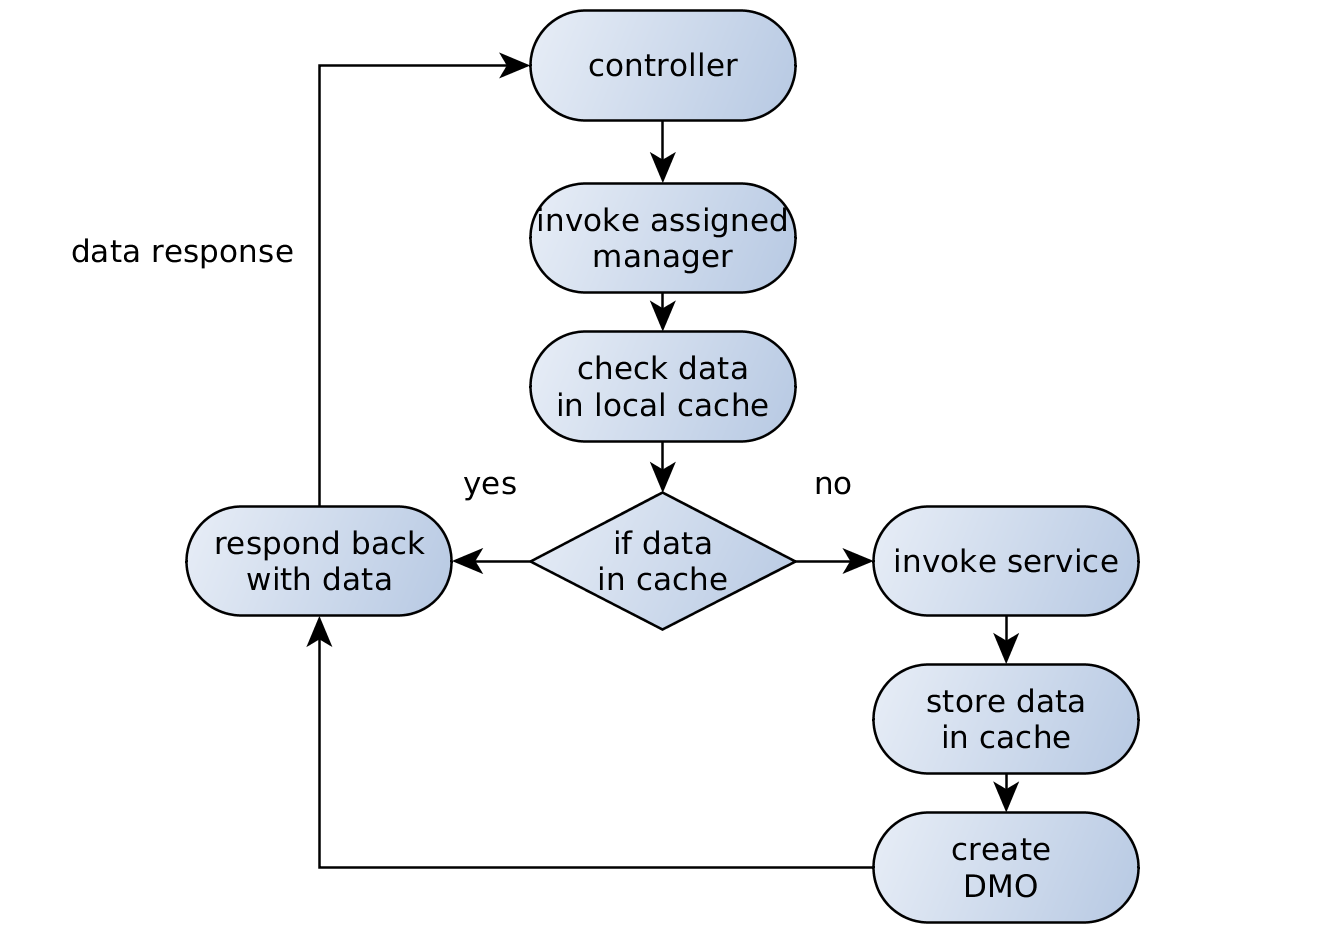
\includegraphics[width=\textwidth]{images/via_manager_1.png}
    \caption{Manager workflow}
    \label{fig:via_manager}
\end{figure}

\begin{figure}[h]
    \centering
	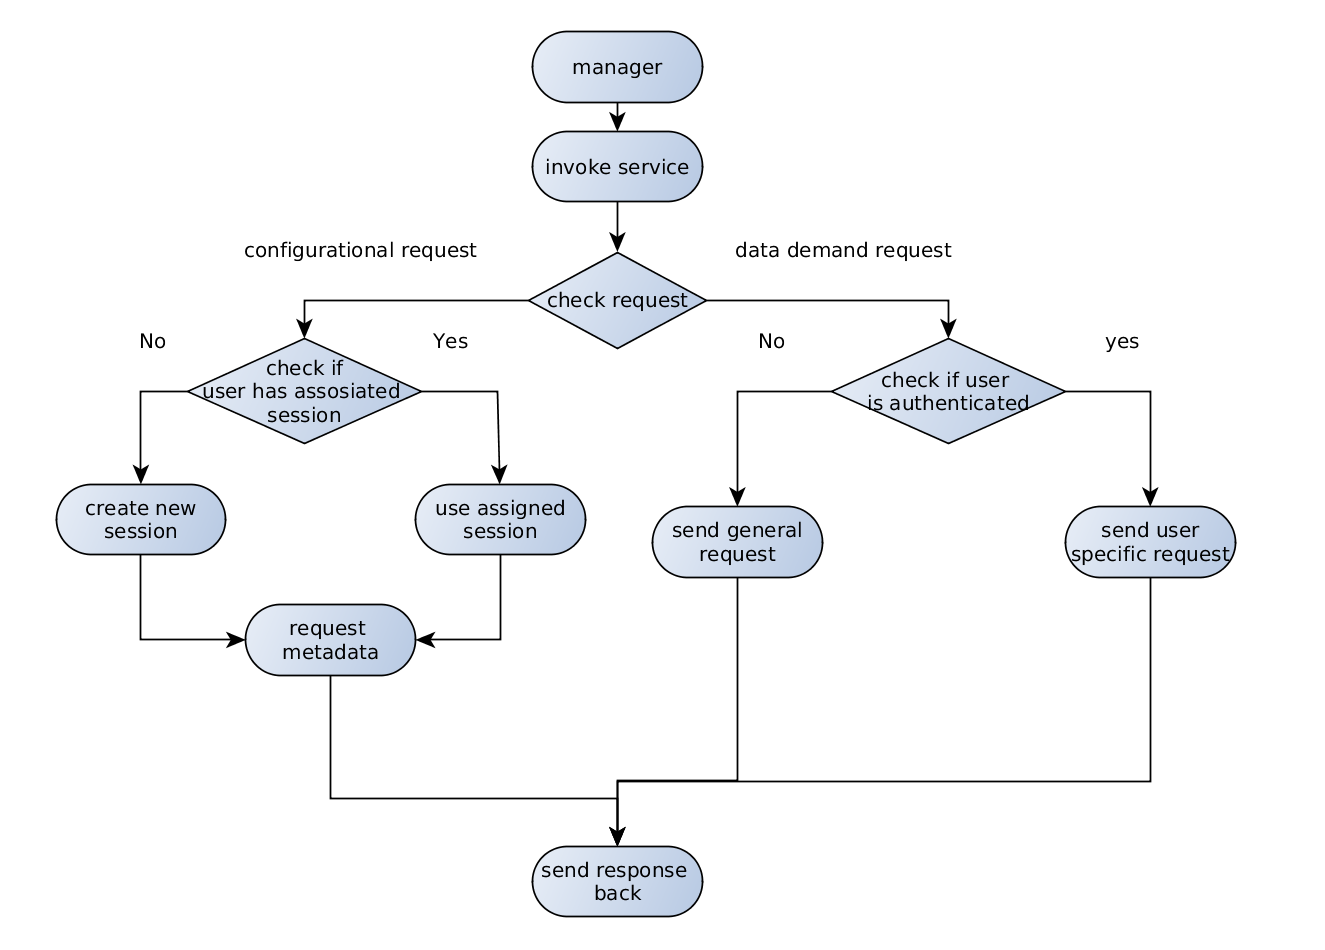
\includegraphics[width=\textwidth]{images/via_service_1.png}
    \caption{Service workflow}
    \label{fig:via_service}
\end{figure}


The client application can make two types of requests: configurational and data demand requests.
The configurational request can have the following purposes:

\begin{itemize}
	\item Provides configuration parameters for both middleware server and client application
	\item Writes user activy
	\item Checks the health of metadata server
	\item Get Content Server url
	\item User settings and preferences
	\item Analytics
\end{itemize}


The data demand request is a request to the content servers. Content servers are customer servers. It means that the response doesn't have predefined structure and can have any structure specified by customer service. 

The controll flow can be described as following: the controller recieves the request from client application, validates data in the request and redirects it to the assigned manager. The middleware server manager invokes corresponding service(i.e. communications layers). When the client application makes the data demand request, the manager invokes content services that redirect request to the assigned content server. The response then is stored in the cache, translated into Data Model Object(DMO) and transferred back to the client in the JSON format. The DMO builders are in charge for translating JSON data into persistent Data Model Objects. For every DMO there is an assigned manager and service. As an example, if the content server responses with video object, there will be VideoManager and VideoService components.   

The client layer and middleware layer are loosely coupled and communicate with each other through REST services. It gives application great flexibility.


\subsection{Session management}

In order to process communication between middleware server and inner servers(metadata server and content distributors), the security layer was implemented(i.e. session management).

The session consists of two parts: 

\begin{itemize}
	\item The client session
	\item The middleware session
\end{itemize}

The purpose of sessions is to distinct users and provide corresponding analytics to the customers.

The client session is represented by the unique session identifier(UID) and the browres id(the string that identifies browser version in the internet). These parameters are generated by the middleware server and transferred to the client through the Set-Cookie header. The browser remembers the data and sends it back with every request in Cookie header.

The session is generated per client when the he makes the initial request. It contains the metadata session key and user session, if the user is authenticated. The metadata session is obtain by making the request to the metadata server. The middleware server sends the aplication key parameter, which is specified in the configuration file and browser id. The metadata server validates the the application key and generates new session for the middleware server. The middleware server assignes this session to the client and stores it locally in memory. Every time when the client will communicate with the middleware server it will send the client's session data. The server will find the metadata session associated with the client and retrieve the medata session. Using this session the middleware can make configurational requests to the metadata session. The sequence diagram of session management is presented on figure \ref{fig:arch_sess_uml}. The application key is given by the system administrator to each middleware server. The browser id can be any string and does not have validation rules.


\begin{figure}[h]
\begin{center}

	\resizebox{1.1\textwidth}{0.5\textwidth} {

	\begin{sequencediagram}
	\newthread[white]{cl}{Client}
	\newinst[1.5]{md}{Middleware server}
	\newinst[3.0]{mt}{Metadata server}

	\begin{call}{cl}{RequestSession}{md}{Client session}

		\begin{call}{md}{GenerateSessionId}{md}{ClienSessionId} \end{call}
		\begin{call}{md}{GenerateBrowserId}{md}{BrowserId} \end{call}
		\begin{call}{md}{RequestMetadataSession}{mt}{MetadataSession} 
			\begin{call}{mt}{ValidataeData}{mt}{}\end{call}
		\end{call}

	\end{call}

	\end{sequencediagram}
	}

\end{center}
\caption{Sequence Diagram of Middleware Session generation}
\label{fig:arch_sess_uml}
\end{figure}


\subsection{Drawbacks of the current architecture}

After careful examination, two categories of problems were defined: Client application drawbacks and Middleware side drawbacks. 

In order to present the page, the client needs to generate a View Model Object(VMO). The VMO contains several Data Model objects(DMOs). The client makes request for every DMO, aggregates the response, generates VMO from DMOs and renders it to the html view. The drawback is that the client has to make several HTTP requests in order to generate single VMO. It would be better for client to make a request for VMO instead of DMO. This approach has several advantages: the client will make less HTTP requests, that will increase the performance by reducing the latency, it will simplify the client logic, because the client will not be requered to generate VMOs from DMOs. 

Another problem with the current client implementation is that it is not generic. If the new content server will be introduced, a lot of code have to be changed on the client side in order to impelment the new logic.

The client can maintain the caching layer that will cache VMOs from the responses. 

The client implements MVC pattern, which produces dublication with middleware server. This approach increases the complexity of the system, the developers should support boch client and middleware MVC applications. We can simplify client and assign two tasks to it: caching and rendering VMOs.

On the middleware side, the DMOs are not generic. The purpose of the middleware server is to serve as a transparent layer, but without dynamic DMO generation a lot of code has to be changed when the new content server is introduced.

The middleware cache can be replaced by the Content Delivery Network(CDN). The middleware caches only information that is common for every user. This work can be done by the CDN edge servers. These will decrease the middleware complexity, decrease the cost of maintaining middleware server.


\newpage
